\documentclass[tikz,border=5pt]{standalone}
\usepackage[T1]{fontenc}
\usepackage{lmodern,amsmath}
\begin{document}
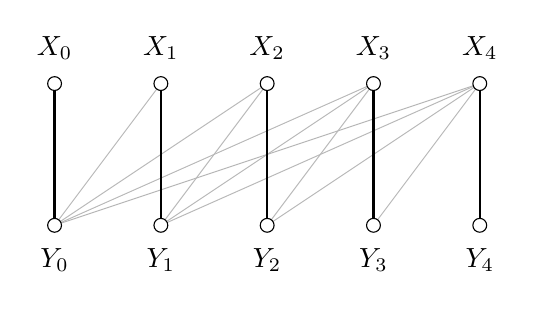
\begin{tikzpicture}[x=1.35cm,y=1cm,
  vertex/.style={circle,draw=black,fill=white,inner sep=0pt,minimum size=5pt}]
\foreach \i in {0,...,4}{
  \coordinate (X\i) at (\i,1.8);
  \coordinate (Y\i) at (\i,0);}
\foreach \i in {0,...,4}{
  \foreach \j in {0,...,4}{
    \ifnum\i>\j\draw[black!28,line width=0.35pt] (X\i)--(Y\j);\fi}}
\foreach \i in {0,...,4}{
  \draw[black,line width=0.9pt] (X\i)--(Y\i);
  \node[vertex] at (X\i) {};
  \node[vertex] at (Y\i) {};
  \node[above=5pt] at (X\i) {$X_{\i}$};
  \node[below=5pt] at (Y\i) {$Y_{\i}$};}
\end{tikzpicture}
\end{document}
